\documentclass[11pt]{article}
\usepackage{graphicx} % Allows including images
\usepackage{booktabs} % Allows the use of \toprule, \midrule and \bottomrule in tables
\usepackage[belowskip=0pt,aboveskip=0pt]{caption}
\usepackage{amsmath}
\usepackage{pifont}
\usepackage{amsthm}
\usepackage{caption}
\usepackage[]{epstopdf}
\usepackage{braket}
%\usepackage{color}
\usepackage{mathtools}


\usepackage{listings}
\lstdefinestyle{mystyle}{
%    backgroundcolor=\color{backcolour},   
%    commentstyle=\color{codegreen},
%    keywordstyle=\color{magenta},
%    numberstyle=\tiny\color{codegray},
%    stringstyle=\color{codepurple},
    basicstyle=\footnotesize,
    breakatwhitespace=false,         
    breaklines=true,                 
    captionpos=b,                    
    keepspaces=true,                 
    numbers=left,                    
    numbersep=5pt,                  
    showspaces=false,                
    showstringspaces=false,
    showtabs=false,                  
    tabsize=2
}
 
\lstset{style=mystyle}


\usepackage{caption}

\usepackage{amsthm,amssymb,graphicx,graphicx,multirow,amsmath,cite}
\usepackage{float}
\usepackage{hyperref}
%\usepackage{minted} %Python Pygments
%\usepackage{listings}
\usepackage[usenames,dvipsnames]{color}
\usepackage{etoolbox}
\include{notation}
\oddsidemargin=0.15in
\evensidemargin=0.15in
\topmargin=-.5in
\textheight=9in
\textwidth=6.25in
%\bootrue{Advanced}

\newtheorem{lemma}{Lemma}{}
  \newtheorem{thm}{Theorem}
  \newtheorem{theorem}{Theorem}
  \newtheorem{prop}{Proposition}
  \newtheorem{cor}[thm]{Corollary}
  \newtheorem{defi}[thm]{Definition}
  \newtheorem{definition}[thm]{Definition}
  
  %% USE THESE IN YOUR TEX CODE.
\def\E{\mathbb{E}} % For Expectation
\def\P{\mathbb{P}} % for probabiltiy
\def\EE{\mathbb{E}^{!o}} % For Palm expectation
\def\ie{{\em i.e.}} 
\def\eg{{\em e.g.}}
\def\V{\operatorname{Var}}
\def\L{\mathcal{L}} % For Laplace transform
\def\i{\mathbf{1}} % Indicator random variable
\def\l{\ell}% For path loss moel


\definecolor{mygreen}{rgb}{0,0.6,0}
\definecolor{mygray}{rgb}{0.5,0.5,0.5}
\definecolor{mymauve}{rgb}{0.58,0,0.82}

\lstset{ %
  backgroundcolor=\color{white},   % choose the background color
  basicstyle=\footnotesize,        % size of fonts used for the code
  breaklines=true,                 % automatic line breaking only at whitespace
  captionpos=b,                    % sets the caption-position to bottom
  commentstyle=\color{mygreen},    % comment style
  escapeinside={\%*}{*)},          % if you want to add LaTeX within your code
  keywordstyle=\color{blue},       % keyword style
  stringstyle=\color{mymauve},     % string literal style
}



\begin{document}
%--------------
%% preamble.tex
%% this should be included with a command like
%% %--------------
%% preamble.tex
%% this should be included with a command like
%% %--------------
%% preamble.tex
%% this should be included with a command like
%% \input{preamble.tex}
%% \lecture{1}{September 4, 1996 }{Daniel A. Spielman}{name
%%  of poor scribe}

\hbadness=10000
\vbadness=10000

\setlength{\oddsidemargin}{.25in}
\setlength{\evensidemargin}{.25in}
\setlength{\textwidth}{6in}
\setlength{\topmargin}{-0.4in}
\setlength{\textheight}{8.5in}

\newcommand{\handout}[5]{
   \renewcommand{\thepage}{#1-\arabic{page}}
   \noindent
   \begin{center}
   \framebox{
      \vbox{
    \hbox to 5.78in { {\b APPM7440: Radial Basis Functions - Finite Differences

 }
     	 \hfill #2 }
       \vspace{4mm}
       \hbox to 5.78in { {\Large \hfill #5  \hfill} }
       \vspace{2mm}
       \hbox to 5.78in { {\it #3 \hfill #4} }
      }
   }
   \end{center}
   \vspace*{4mm}
}

\newcommand{\lecture}[4]{\handout{#1}{#2}{ #3}{Scribe: #4}{ Lecture #1}}
\newcommand{\assignment}[5]{\handout{#1}{#2}{ #3}{Author: #4(#5)}{ Assignment #1}}
\newcommand{\labreport}[5]{\handout{#1}{#2}{ #3}{Author: #4(#5)}{ Lab Report #1}}
%% \lecture{1}{September 4, 1996 }{Daniel A. Spielman}{name
%%  of poor scribe}

\hbadness=10000
\vbadness=10000

\setlength{\oddsidemargin}{.25in}
\setlength{\evensidemargin}{.25in}
\setlength{\textwidth}{6in}
\setlength{\topmargin}{-0.4in}
\setlength{\textheight}{8.5in}

\newcommand{\handout}[5]{
   \renewcommand{\thepage}{#1-\arabic{page}}
   \noindent
   \begin{center}
   \framebox{
      \vbox{
    \hbox to 5.78in { {\b APPM7440: Radial Basis Functions - Finite Differences

 }
     	 \hfill #2 }
       \vspace{4mm}
       \hbox to 5.78in { {\Large \hfill #5  \hfill} }
       \vspace{2mm}
       \hbox to 5.78in { {\it #3 \hfill #4} }
      }
   }
   \end{center}
   \vspace*{4mm}
}

\newcommand{\lecture}[4]{\handout{#1}{#2}{ #3}{Scribe: #4}{ Lecture #1}}
\newcommand{\assignment}[5]{\handout{#1}{#2}{ #3}{Author: #4(#5)}{ Assignment #1}}
\newcommand{\labreport}[5]{\handout{#1}{#2}{ #3}{Author: #4(#5)}{ Lab Report #1}}
%% \lecture{1}{September 4, 1996 }{Daniel A. Spielman}{name
%%  of poor scribe}

\hbadness=10000
\vbadness=10000

\setlength{\oddsidemargin}{.25in}
\setlength{\evensidemargin}{.25in}
\setlength{\textwidth}{6in}
\setlength{\topmargin}{-0.4in}
\setlength{\textheight}{8.5in}

\newcommand{\handout}[5]{
   \renewcommand{\thepage}{#1-\arabic{page}}
   \noindent
   \begin{center}
   \framebox{
      \vbox{
    \hbox to 5.78in { {\b APPM7440: Radial Basis Functions - Finite Differences

 }
     	 \hfill #2 }
       \vspace{4mm}
       \hbox to 5.78in { {\Large \hfill #5  \hfill} }
       \vspace{2mm}
       \hbox to 5.78in { {\it #3 \hfill #4} }
      }
   }
   \end{center}
   \vspace*{4mm}
}

\newcommand{\lecture}[4]{\handout{#1}{#2}{ #3}{Scribe: #4}{ Lecture #1}}
\newcommand{\assignment}[5]{\handout{#1}{#2}{ #3}{Author: #4(#5)}{ Assignment #1}}
\newcommand{\labreport}[5]{\handout{#1}{#2}{ #3}{Author: #4(#5)}{ Lab Report #1}}
\labreport{4}{April 30, 2015}{Homework 4}{Prasanth Prahladan}{100817764}

\section{Time-Independent PDE}
Attempt to reproduce Figure 4.4(a) in text book, with a node-distribution similar to that in Figure 4.3(c).

\subsection{Derivation of Laplacian}

\begin{align*}
\Phi(r) &= \Phi(\sqrt(x^2 + y^2))\\
\Delta\Phi &= \frac{\partial^2}{\partial^2 x^2 } + \frac{\partial^2}{\partial^2 y^2}\\
\frac{\partial^2 \Phi}{\partial^2 x^2 } & = \big(\frac{\partial r}{\partial x }\big)^2 \big( \frac{\partial^2 \Phi}{\partial^2 r^2} - \frac{1}{r} \frac{\partial \Phi}{\partial r} \big)\\
\frac{\partial^2 \Phi}{\partial^2 y^2 } & = \big(\frac{\partial r}{\partial y }\big)^2 \big( \frac{\partial^2 \Phi}{\partial^2 r^2} - \frac{1}{r} \frac{\partial \Phi}{\partial r} \big)\\
\end{align*}
We thus derive, the relationship for the Laplacian of the RBF
\begin{align}
\Delta\Phi &= \big( \frac{\partial^2}{\partial^2 x^2 } + \frac{\partial^2}{\partial^2 y^2} \big) \Phi\\
&= \big( \frac{\partial^2 }{\partial^2 r^2} - \frac{1}{r} \frac{\partial }{\partial r} \big)\Phi
\end{align}

For the different families of RBF-functions we derive the following
\begin{enumerate}
\item Gaussian RBF
\begin{align}
\Phi(r) &= e^{-(\epsilon r)^2}\\
\Delta\Phi(r) &= 4\epsilon^4 r^2 e^{-(\epsilon r)^2}
\end{align}

\item Multi-quadratic(MQ)
\begin{align}
\Phi(r) &= \sqrt{1 + (\epsilon r)^2}\\
\Delta \Phi(r) &= - (\epsilon r)^2 \big( 1 + (\epsilon r)^2\big)^{-3/2}
\end{align}

\item Inverse Quadratic(IQ)
\begin{align}
\Phi(r) &= \frac{1}{1 + (\epsilon r)^2}\\
\Delta\Phi(r) &= 8\epsilon^4 \frac{r^2}{\big(1 + (\epsilon r)^2\big)^3}
\end{align}



\end{enumerate}


\subsection{Plots generated}


\begin{figure}[h!]
\centering
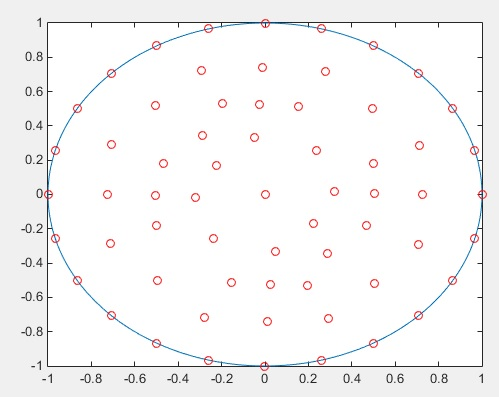
\includegraphics[scale=0.7]{nodeDist.jpg}\\
\caption{Node Distribution in Disc}
\label{fig:NodeDistribution}
\end{figure}


\begin{figure}[h!]
\centering
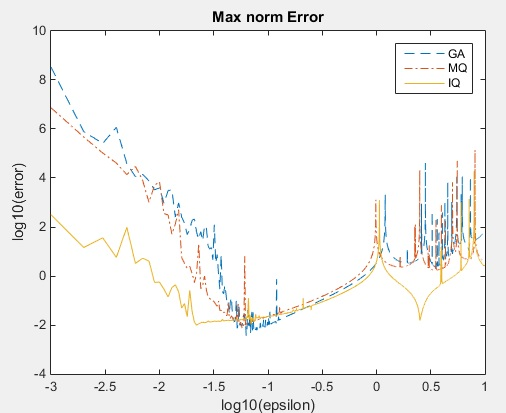
\includegraphics[scale=0.7]{pdeTimeInvariant.jpg}\\
\caption{Max Norm Error variation with epsilon}
\label{fig:errorPDEspatial}
\end{figure}


\subsection{Matlab Implementation}
\begin{lstlisting}[language=octave]
% Code to reproduce Fig 4.4(a) using Matlab PDE Toolbox - Mesh Generating
% function to create Mesh in Fig 4.3(c)

clear all
close all

bndryN = 16;
intrN = 48;
totalN = bndryN + intrN;

% % =======================================================================
% % =======================================================================
% Determine the Test Points 
r = 0.3;
[p,e,t] = initmesh('circleg','Hmax',r); % create Circular Mesh with 64 points
tstX = p(1,:)';
tstY = p(2,:)';
% % =======================================================================
% Determine the Points of Grid
r = 0.35;
[p,e,t] = initmesh('circleg','Hmax',r); % create Circular Mesh with 64 points

% p : DESIRED CIRCULAR MESH for RBF INTERPOLATION.
gridX = p(1,:)';
gridY = p(2,:)';

% ------------------------------------------------------
% plot Unit Circle
theta = 0:0.01:2*pi;
x = cos(theta);
y = sin(theta);
fig1 = figure(1)
plot(x,y)
hold on
% plot the mesh-points
scatter(gridX, gridY,'r')
hold off

% % =======================================================================
    % % =======================================================================
    %[g f] = evalPDEatPoints(p);
    % --------------------------------------------
    % g = u(x,y) =  A ./ (A + (x - a).^2 + b* y.^2);
    % f = Laplacian[u(x,y)] = -2*A*(A + (x - a).^2 + b* y.^2).^(-3)
    % .*(A(b+1) + (x-a)^2(b-3) + y^2(b -3b^2))
    % --------------------------------------------
    % Boundary Constraint
    g = @(X, Y) (100 ./(100 + (X - 0.2).^2 + 2* Y.^2) );
    % Interior Constraint
    f = @(X,Y) (-2*100*(100*(2+1) + (2-3)*(X-0.2).^2 + (2 - 3*2^2)*Y.^2).*(100 + (X - 0.2).^2 + 2*Y.^2).^(-3));
    
    
% % =======================================================================
% % =======================================================================
% Solving PDE using RBF
        

epsilons = 0.001:0.001:10;
maxError = zeros(length(epsilons),3);

for i = 1:3
    switch i
        case 1
            rbf = 'GA'
        case 2
            rbf = 'IQ'
        case 3 
            rbf = 'MQ'
    end

for count = 1:length(epsilons)
    ep = epsilons(count);
   
    % % =======================================================================
    % % =======================================================================
    % Kansa's Formulation
    % --------------------------------------------------
    % Determine Vectors
    
    gridR = gridX.^2 + gridY.^2;
    
    % Identify index of points that are located on UNIT CIRCLE BOUNDARY
    bdryID = find(gridR==1);
    intrID = find(gridR<1);
    
    % Rearrange Points such that first values are on Boundary and remaining
    % are in the interior
    
    newOrder = [bdryID; intrID];
    gridX = gridX(newOrder);
    gridY = gridY(newOrder); 
    
    numBoundaryPts = length(bdryID);
    
    % Evaluate Boudary Constraint
    gridX_BND = gridX(1:numBoundaryPts);
    gridY_BND = gridY(1:numBoundaryPts);
    gGrid = g(gridX_BND,gridY_BND);
    
    % Evaluate Interior Constraint
    gridX_INT = gridX(numBoundaryPts +1:end);
    gridY_INT = gridY(numBoundaryPts +1:end);
    fGrid = f(gridX_INT,gridY_INT);
        
    % ---------------------------------------------------
    % Compute R for the A matrix
    
    [x1, x2] = meshgrid(gridX);
    [y1, y2] = meshgrid(gridY);
    d2 = (x1 - x2).^2 + (y1 - y2).^2;
    r = sqrt(d2);
    
    % Generate the A matrix for points on Boundary
    A = fi(rbf,ep, r(1:numBoundaryPts,:) );
    % Generate Laplacian_A matrix for points in Interior
    LA = Lfi(rbf,ep, r(numBoundaryPts+1:end,:) );
    
    % Matrix for Kansa's Method
    Ahat = [A; LA];
    
    % Evaluate the weighting coefficients
    lambda = Ahat\[gGrid;fGrid];
    
    % Grid points tst_i - grid_j
    [tX gX] = ndgrid(tstX, gridX);
    [tY gY] = ndgrid(tstY, gridY);
    
    tstR2 = (tX-gX).^2 + (tY - gY).^2;
    tstR = sqrt(tstR2);
    
    
    tstA = fi(rbf,ep,tstR);
    
%     fprintf('tstU_rbf\n')
    tstU_rbf = tstA*lambda;
    size(tstU_rbf);
    
%     fprintf('tstU_true\n')
    tstU_true = g(tstX,tstY);
    size(tstU_true);
    
    error = tstU_true - tstU_rbf;
    maxError(count,i) = max(abs(error));
end

end
fig2 = figure(2)
plot(log10(epsilons),log10(maxError(:,1)),'--',log10(epsilons),log10(maxError(:,2)),'-.', log10(epsilons),log10(maxError(:,3)),'-' )
title('Max norm Error')
xlabel('log10(epsilon)')
ylabel('log10(error)')
legend('GA','MQ','IQ')

% ==============================================================================
% Computation of Laplacian of RBF
function LPhi = Lfi(type,ep,r)

switch type
    case 'GA'
    % Gaussian RBF
    LPhi =  ( 4*ep^4*r.^2.*exp(-(ep*r).^2));      
    
    case 'MQ'
    % MQ
    LPhi =  -(ep*r).^2.*(1 + (ep*r).^2).^(-3/2);  
        
    case 'IQ'
    % IQ
    LPhi = (8*ep^4*r.^2.*(1 + (ep*r).^2).^(-3) ); 

end
end

% ==============================================================================
% RBF Function computation
function Phi = fi(type,ep,r)
switch type
    case 'GA'
    % Gaussian RBF
    Phi = (exp(-(ep*r).^2));
    
    case 'MQ'
    % MQ
    Phi = (1 + (ep*r).^2).^(1/2);    
        
    case 'IQ'
    % IQ
    Phi = (1 + (ep*r).^2).^(-1);    
end
end
\end{lstlisting}


\section{Time-dependent PDE: Global RBF}
Solid body convection around a Unit Sphere

\begin{align}
\frac{\partial h}{\partial t} &= -\big( \frac{u}{a \cos\theta} \frac{\partial}{\partial \phi} + \frac{v}{a} \frac{\partial}{\partial\theta} \big) h \\
u &= u_0 (\cos\theta \cos\alpha - \sin\theta \sin\theta \sin\phi \sin\alpha)\\
v &= u_0 \cos\phi \sin\alpha
\end{align}

In the given exercise, we choose $u_0/a = 1 = 2\pi /T$, where $T$ is the Time Period of revolution around the sphere. 
For the specific case of simulations related to the earth, we have $a$ represents the radius of the earth, and $T = 12$ days.

\subsection{Initial Conditions on Sphere}
Cosine bell function
\begin{align}
h(\theta, \phi) = \bigg\lbrace\begin{array}{cc}
\frac{h_0}{2}\big(1 + cos(\frac{\pi r}{R})\big) & r< R\\
0 & r \geq R
\end{array}
\end{align}

\begin{align}
r &= a \cos^{-1}\big( \sin\theta_c \sin\theta + \cos\theta_c \cos\theta \cos(\phi - \phi_c) \big)\\
R &= a/3 \notag \\
h_0 &= 1 \notag \\
(\theta_c, \phi_c) &= (0,0). \notag
\end{align}

\subsection{Derivation of the method of applying RBF for solving the PDE}
The system if solved as follows. We represent the time-varying PDE as follows.
\begin{align*}
\frac{dh}{dt} &= - \big( \frac{u}{\cos\theta} \frac{\partial}{\partial \phi} + v \frac{\partial}{\partial\phi}\big) h(\theta,\phi) \\
\frac{dh}{dt} &= - L(h)
\end{align*}
Further, we try to derive an RBF based spatial-stencil to approximate the Linear Operator $L$. This involves computing the weights($w$) in the equation:
\begin{align}
[A][w] = [f] = [L \Phi(||x - x_j||) |_{x = x_i}]
\end{align}
which $f$ corresponds to the function we wish to approximate using RBFs. The above equation $[w]$ corresponds to the weights associated with the neighbourhood points, when the stencil is centered at point $x = x_i$.

Since, we have the data given in cartesian coordiantes $(x,y,z)$ we first try to convert the Operator expression into cartesian coordinates, before working with RBFs. Since the Linear Operator,$L$ is given by:
\begin{align}
L = \frac{u}{\cos\theta} \frac{\partial}{\partial \phi} + v \frac{\partial}{\partial\phi} \label{eq:LinearOperator}
\end{align}
we need to compute  $\frac{\partial}{\partial}\Phi(||x - x_j||)$ and $\frac{\partial}{\partial}\Phi(||x - x_j||)$.
\begin{align*}
\phi &\equiv \phi(x,y,z) \\
\theta &\equiv \theta(x,y,z)\\
\frac{\partial}{\partial\phi} &= \frac{\partial}{\partial x}\frac{\partial x}{\partial \phi} + \frac{\partial}{\partial y} \frac{\partial y}{\partial \phi} + \frac{\partial}{\partial z} \frac{\partial z}{\partial \phi} \\
\frac{\partial}{\partial\theta} &= \frac{\partial}{\partial x}\frac{\partial x}{\partial \theta} + \frac{\partial}{\partial y} \frac{\partial y}{\partial \theta} + \frac{\partial}{\partial z} \frac{\partial z}{\partial \theta} \\
\end{align*}

Further, we have the conversion relations from spherical to cartesian coordinates for coordinates on a Unit Sphere
\begin{align*}
x &= \cos\phi\cos\theta \\
y &= \sin\phi \cos\theta \\
z &= \sin\theta \\
\end{align*}
This gives us the following relationships for the terms included in the above equation
\begin{align*}
\begin{array}{cc}
\frac{\partial x}{\partial \phi} = -\sin\phi \cos\theta & \frac{\partial x}{\partial \theta} = -\cos\phi\sin\theta\\
\frac{\partial y}{\partial \phi} = \cos\theta \cos\phi& \frac{\partial y}{\partial \theta} = -\sin\phi \sin\theta\\
\frac{\partial z}{\partial \phi}= 0 & \frac{\partial z}{\partial \theta} = \cos\theta.
\end{array}
\end{align*}
Further, we also have the relation $r^2 = (x - x_i)^2 + (y - y_i)^2 + (z- z_i)^2$, from which we derive 
\begin{align*}
\frac{\partial r}{\partial x} = \frac{x - x_i}{r}\\
\frac{\partial r}{\partial y} = \frac{y - y_i}{r}\\
\frac{\partial r}{\partial z} = \frac{z - z_i}{r}.
\end{align*}
Substituting, all the above expansion into the equation for Linear Operator $L$ \eqref{eq:LinearOperator} obtain its
representation in cartesian-coordinates. Further, we proceed to evaluate the cartesian-coordinate based respresentation of the Operator applied to the RBF-approximation of function (solution of PDE, $h(x,y,z,t)$) under study.

The weight$[w_i]$ vectors computed for each stencil centered at $x_i$ form the rows of the Differentiation Matrix. 

For solving the time-varying PDE, we use an RK4 based time-integrator to solve the following ODE
\begin{align}
\frac{d h(x,y,z,t)}{dt}  = -[DM] h(x,y,z,t)
\end{align}
where, $[DM]$ is the Differentiation Matrix computed using the code provided in the course-website.

For stability of the time-integration, we need to ensure that the eigenvalues of the Differentiation Matrix,$[DM]$ , should be contained within the stability-domain of time-integrator for the given choice of time-step. 

\subsection{Matlab Code Implementation}

\subsubsection{Time-stepping using RK4}
\begin{lstlisting}[language=octave]

% -------------------------------------------------------------------------
% -------------------------------------------------------------------------
% PDE - TIME STEPPING
% -------------------------------------------------------------------------
% -------------------------------------------------------------------------

% Convert from Cartesian Coordinates to Spherical Cordinates
ptsXYZ = xyz(:,1:3);
ptsX = xyz(:,1);
ptsY = xyz(:,2);
ptsZ = xyz(:,3);

Phi = xyz(:,4);
The = xyz(:,5);

% -------------------------------------------------------------------------
% Plot the Cosine Bell Function
m = 0:0.01:1;
R = 1/3;
h0 = 1;
ratio = m/R;
indx = (ratio<1);
hfun  = h0/2*(1+cos(pi.*ratio)).*indx;
fig2 = figure(2)
plot(m,hfun)
xlabel('r')
ylabel('Cosine Bell: h(r)')

% Evaluate the Cosine Bell for Initial Condition
r = acos(cos(The).*cos(Phi));
ratio = r/R;
indx = (ratio<1);
initH  = h0/2*(1+cos(pi.*ratio)).*indx;         % Initialize Function

% -------------------------------------------------------------------------
% Plotting using RegularizeData3D (Matlab Central)
theta = -2:0.1:2;
phi = -3.5:0.1:3.5;
Smoothness = 0.00005;

fig4 = figure(4)
z0 = RegularizeData3D(The,Phi,initH, theta, phi, 'interp', 'bicubic', 'smoothness', Smoothness);
surf(theta, phi, z0, 'facealpha', 0.50);
hold on
scatter3(The,Phi,initH, 'fill');
hold off
xlabel('\theta')
ylabel('\phi')
zlabel('h(\theta,\phi,t = 0)')
title('Initialization of Cosine Bell Curve')
% -------------------------------------------------------------------------
% -------------------------------------------------------------------------
% Time-Step using RK4
fractionOfRevolution = 1000;            % Ensure divisible by 4
T1rev = 2*pi;
t0 = 0;
tf = (10)*T1rev; % around 100 revolutions
dT = T1rev/fractionOfRevolution;
[t,H] = rk4_hw4(@fun_dudt_hw4, t0:dT:tf, initH, ptsXYZ);  

% -------------------------------------------------------------------------
% -------------------------------------------------------------------------
% Plots of Time-Revolution: RegularizeData3D (Matlab Central FileID: #46223)

fig10 = figure(10)
subplot(2,2,1)
data = initH;
z0 = RegularizeData3D(The,Phi,data, theta, phi, 'interp', 'bicubic', 'smoothness', Smoothness);
surf(theta, phi, z0, 'facealpha', 0.50);
hold on
scatter3(The,Phi,data, 'fill');
hold off
xlabel('\theta')
ylabel('\phi')
zlabel('h(\theta,\phi,t)')
title('Initialization of Cosine Bell Curve')
% -------------------------------
subplot(2,2,2)
data = H(:,fractionOfRevolution/4);
zHalfT = RegularizeData3D(The,Phi,data, theta, phi, 'interp', 'bicubic', 'smoothness', Smoothness);
surf(theta, phi, zHalfT, 'facealpha', 0.50);
hold on
scatter3(The,Phi,data,'fill')
hold off
xlabel('\theta')
ylabel('\phi')
zlabel('h(\theta,\phi,t)')
title('PDE Solution @t = T/4')
% -------------------------------
subplot(2,2,3)
data = H(:,2*fractionOfRevolution/4);
zHalfT = RegularizeData3D(The,Phi,data, theta, phi, 'interp', 'bicubic', 'smoothness', Smoothness);
surf(theta, phi, zHalfT, 'facealpha', 0.50);
hold on
scatter3(The,Phi,data,'fill')
hold off
xlabel('\theta')
ylabel('\phi')
zlabel('h(\theta,\phi,t)')
title('PDE Solution @t = T/2')
% -------------------------------
subplot(2,2,4)
data = H(:,3*fractionOfRevolution/4);
zHalfT = RegularizeData3D(The,Phi,data, theta, phi, 'interp', 'bicubic', 'smoothness', Smoothness);
surf(theta, phi, zHalfT, 'facealpha', 0.50);
hold on
scatter3(The,Phi,data,'fill')
hold off
xlabel('\theta')
ylabel('\phi')
zlabel('h(\theta,\phi,t)')
title('PDE Solution @t = 3*T/4')
% -------------------------------
% Plot Error after full revolution
fig11 = figure(11)
error = abs(H(:,fractionOfRevolution) - initH);
data = error;
Smoothness = 0.00005;

zFullT = RegularizeData3D(The,Phi,data, theta, phi, 'interp', 'bicubic', 'smoothness', Smoothness);
surf(theta, phi, zFullT, 'facealpha', 0.75);
hold on
scatter3(The,Phi,data,'fill')
hold off
xlabel('\theta')
ylabel('\phi')
zlabel('error(\theta,\phi,t)')
title('Error after 1 revolutions')

% -------------------------------
% Plot Error after 10 full revolution
fig12 = figure(12)
error = abs(H(:,end) - initH);
data = error;
Smoothness = 0.00005;

zFullT = RegularizeData3D(The,Phi,data, theta, phi, 'interp', 'bicubic', 'smoothness', Smoothness);
surf(theta, phi, zFullT, 'facealpha', 0.75);
hold on
scatter3(The,Phi,data,'fill')
hold off
xlabel('\theta')
ylabel('\phi')
zlabel('error(\theta,\phi,t)')
title('Error after 10 revolutions')

%====================================================================


\end{lstlisting}



\subsection{Simulations and results after 1/2, 1 and 10 revolutions around sphere}
It is noted that after about 10 revolutions error of the order of $3$ percent is observed.  The graphs show the time-evolution of the cosine bell curve. 


\begin{figure}[h!]
\centering
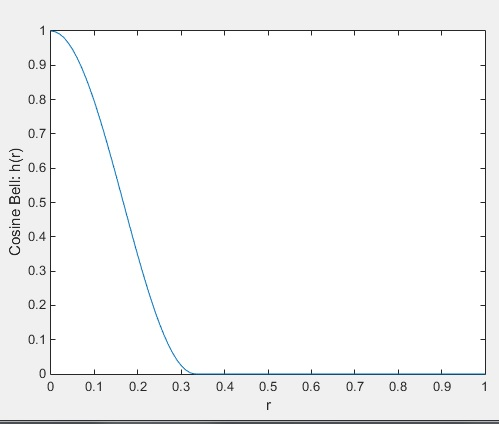
\includegraphics[scale=0.7]{CosineBellGraph.jpg}\\
\caption{Cosine Bell Curve}
\label{fig:CosineBellCurve}
\end{figure}

\begin{figure}[h!]
\centering
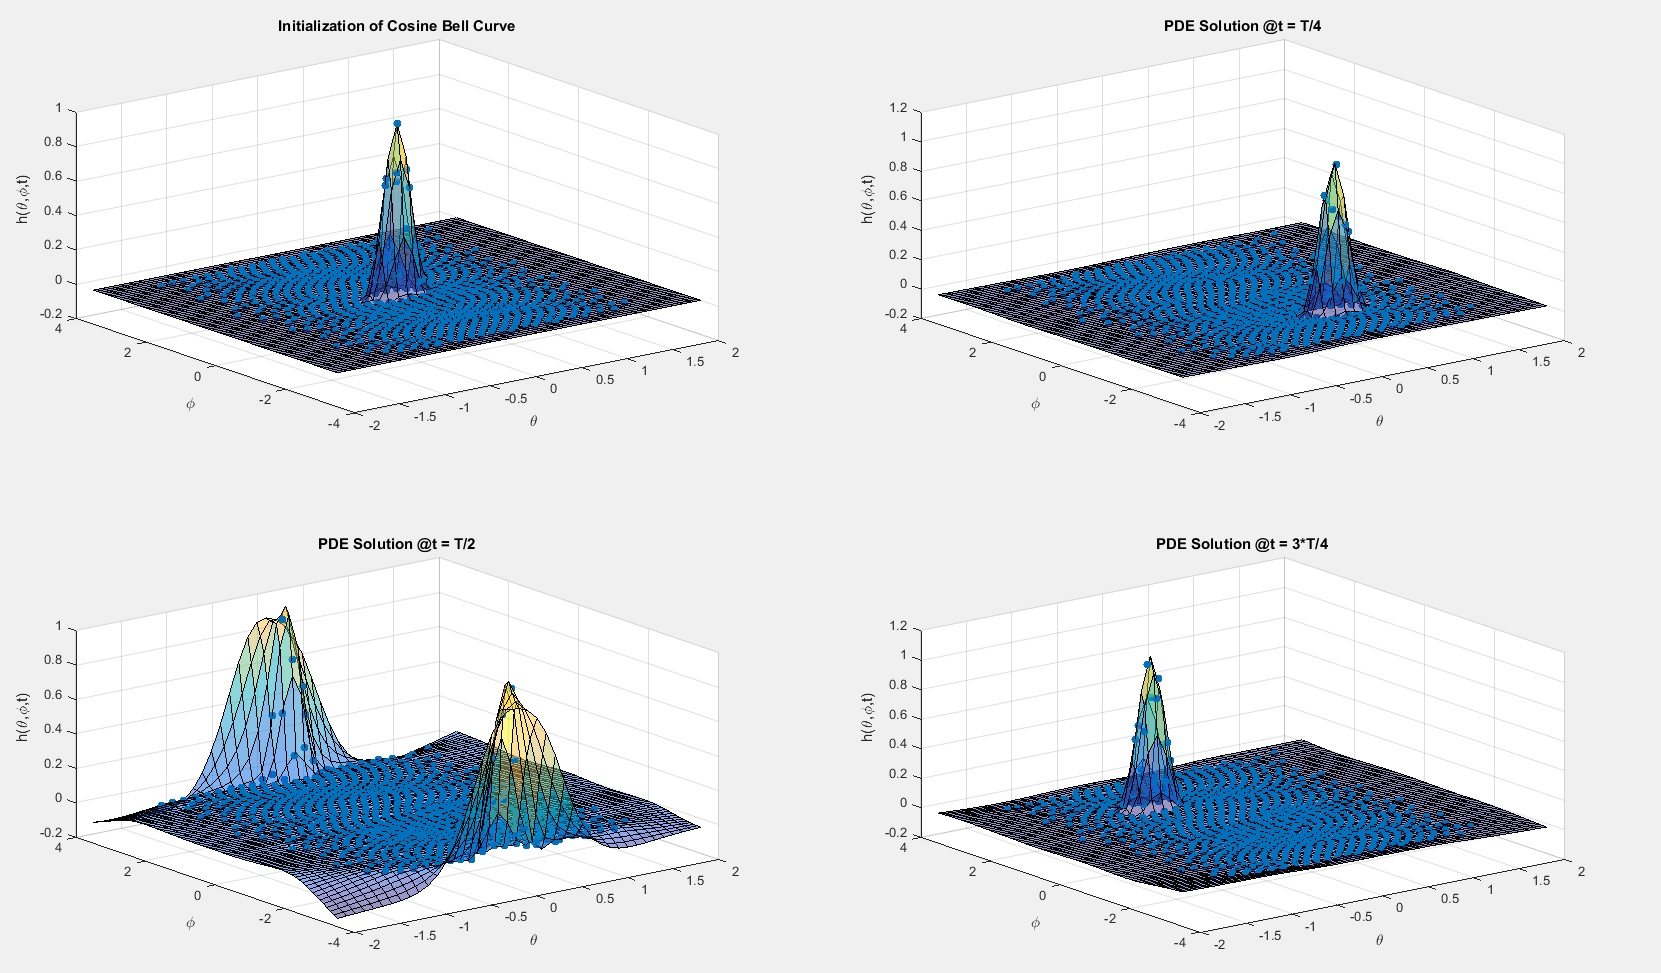
\includegraphics[scale=0.4]{pdeEvolGlobalRBF.jpg}\\
\caption{PDE Evolution over 1 revolution}
\label{fig:PDEvolGlobalRBF}
\end{figure}

\begin{figure}[h!]
\centering
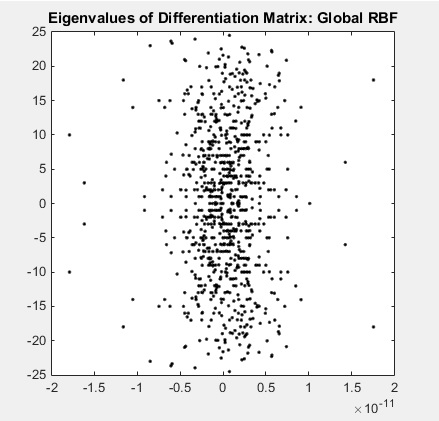
\includegraphics[scale=0.7]{globalRBF_eigenvals.jpg}\\
\caption{Eigenvalues of the Differentiation Matrix}
\label{fig:GlobalRBFevs}
\end{figure}

\begin{figure}[h!]
\centering
\begin{minipage}{.5\linewidth}
  \centering
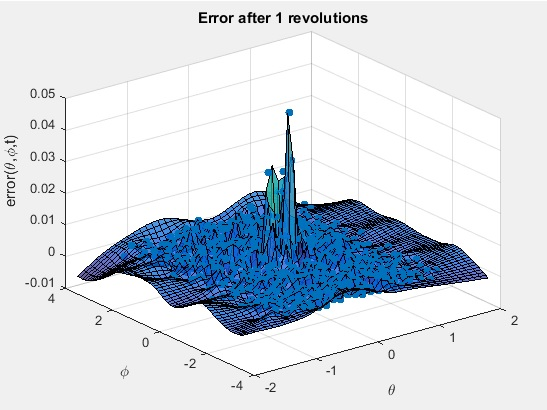
\includegraphics[scale=0.7]{error1rev.jpg}
\label{fig:global1rev}
\captionof{figure}{Errors after 1 rev}
\end{minipage}%

\begin{minipage}{.5\linewidth}
  \centering
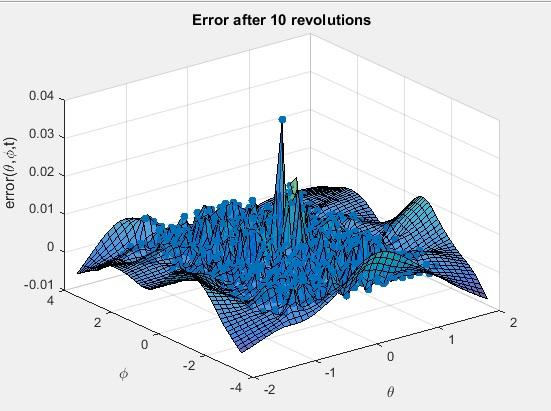
\includegraphics[scale=0.7]{error10rev.jpg}
\label{fig:global10rev}\
\captionof{figure}{Errors after 10 revs}
\end{minipage}
\end{figure}




\section{Time-dependent PDE: RBF- Finite Differences}

For the RBF-FD based approach towards solving the PDE for convection on solid-sphere surface, the derivations are similar. The only major difference is in the choice of a local-stencil which comprises of $n=20$ nearest neighbours of the center-point of the stencil. 

The choice of local stencil leads to creation of a Sparse-Differentiation Matrix. 

We observe that the sparse-DM created by RBF-FD has positive eigenvalues in the Right-Half Complex plane, which leads to instabilities in the time-stepping process. 

\subsection{Structure of RBF-FD Differentiation Matrix}



\begin{figure}[h!]
\centering
\begin{minipage}{.33\hsize}
  \centering
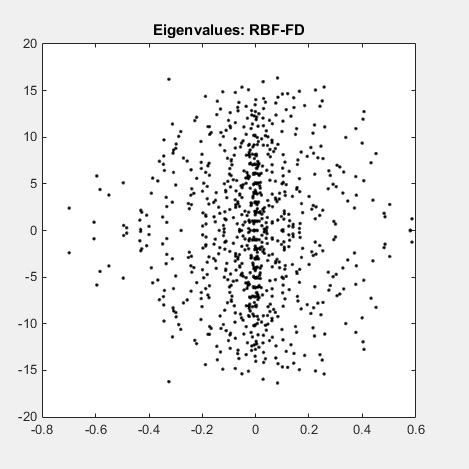
\includegraphics[scale=0.5]{FD_RBF_eigenvals.jpg}
\label{fig:rbfFDeigenvalues}
\captionof{figure}{Eigenvalues of RBF-FD DM}
\end{minipage}%

\begin{minipage}{.33\hsize}
  \centering
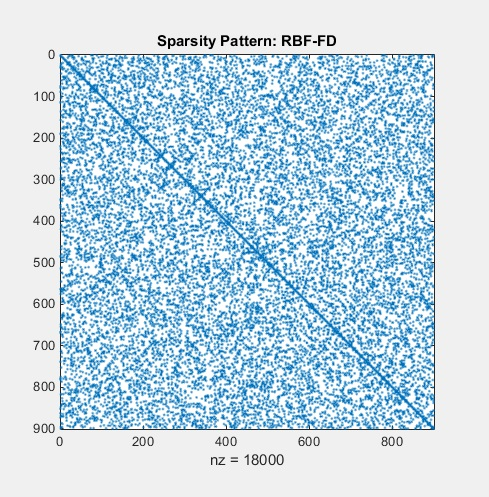
\includegraphics[scale=0.5]{FD_RBF_sparse01.jpg}
\label{fig:rbfFDdiffmat}\
\captionof{figure}{Sparsity Pattern of RBF-FD Differentiation Matrix}
\end{minipage}

\begin{minipage}{.33\hsize}
  \centering
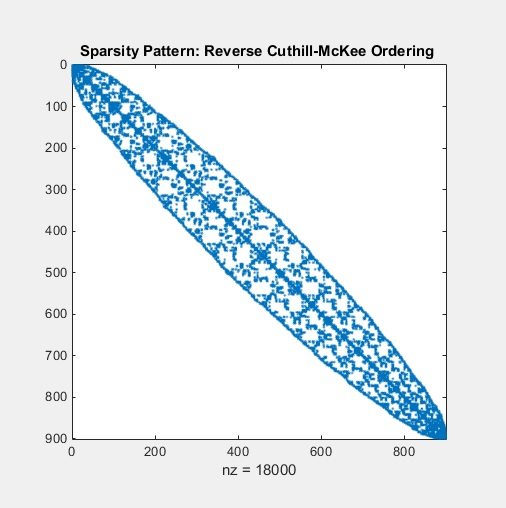
\includegraphics[scale=0.5]{FD_RBF_sparse02.jpg}
\label{fig:rbfFDdiffmatRCM}\
\captionof{figure}{Sparsity Pattern of RBF-FD DM: Reverse Cuthill-McKee Ordering}
\end{minipage}

\end{figure}

\begin{figure}[h!]
\centering
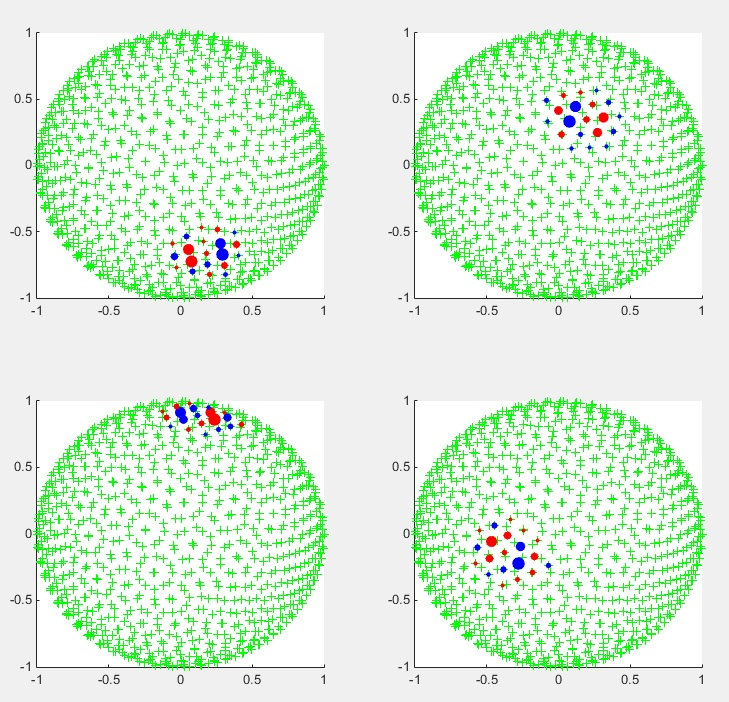
\includegraphics[scale=0.4]{RBF_FD_stencils.jpg}\\
\caption{Plot of Local Stencils}
\label{fig:localStencilWeights}
\end{figure}

\subsection{Simulations and results after 1/2, 1 and 10 revolutions around sphere}
It is observed that RBF-FD simulations become unstable even before completion of 1 revolution around the sphere.
Further, it is to be noted that the present implementation does not consider combination of RBF and Polynomial approximation of the solution. This was because, for $\epsilon = 2$ we noted in class, that using adding polynomial terms does not add significantly to the accuracy.(Figure 5.7 of text-book.)

\begin{figure}[h!]
\centering
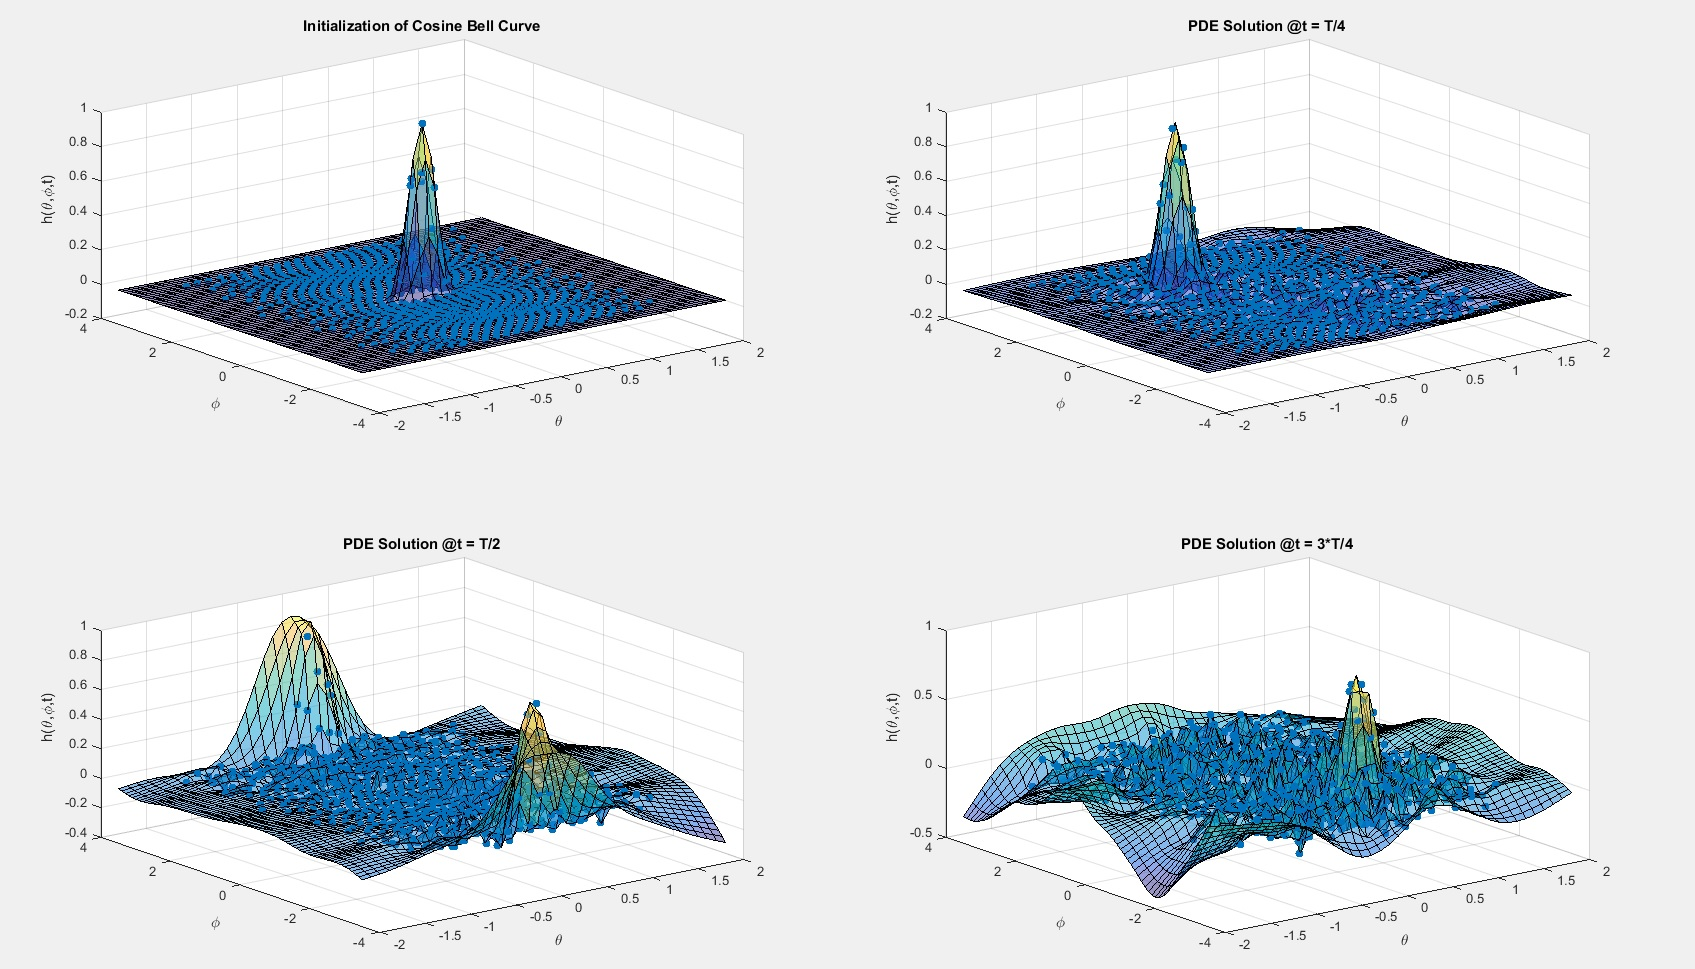
\includegraphics[scale=0.4]{pdeEvolRBF_FD.jpg}\\
\caption{PDE Evolution over 1 revolution}
\label{fig:PDEvolGlobalRBF}
\end{figure}

\begin{figure}[h!]
\centering
\begin{minipage}{.5\textwidth}
  \centering
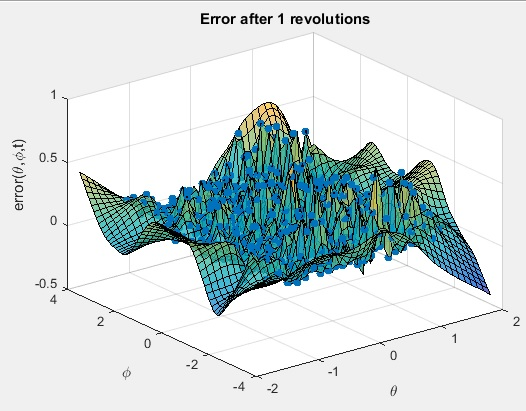
\includegraphics[scale=0.7]{error1rev_FD.jpg}
\label{fig:global1rev}
\captionof{figure}{Errors after 1 rev}
\end{minipage}%

\begin{minipage}{.5\textwidth}
  \centering
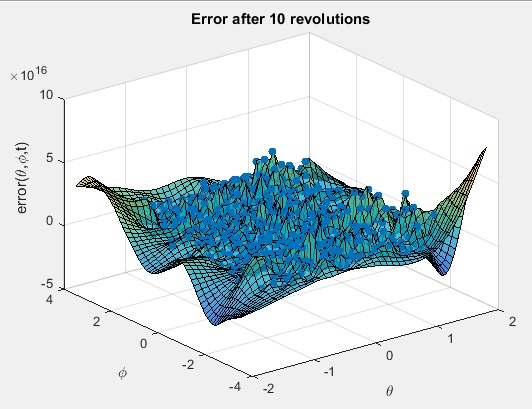
\includegraphics[scale=0.7]{error10revFD.jpg}
\label{fig:global10rev}\
\captionof{figure}{Errors after 10 revs}
\end{minipage}
\end{figure}

\subsection{Matlab Code Implementation}

\subsubsection{Time-stepping using RK4}
\begin{lstlisting}[language=octave]
% RBF-FD Differentiation Matrix
global D;       
D = zeros(N,N);
D = sparse(D);

% Determine n-nearest neighbors
n = 20;
IDX = knnsearch(xyz(:,1:3),xyz(:,1:3),'K',n,'Distance','euclidean');

for i = 1:N % Evaluate L at xyz(i,:) when RBF centered at xyz(j,:), j=1:m
            % Note that we only need a single loop
            
    nbrs = IDX(i,:);
    
    % Compute values only to particular neighbors
    dx_dfi = -xyz(i,7)*xyz(i,8);        % To obtain the weights (which form 
    dy_dfi =  xyz(i,6)*xyz(i,8);        % the rows of the DM) we need  
    dz_dfi =  0;                        % for each RBF to calculate its
                                        % derivatives at node i with
    dx_dth = -xyz(i,6)*xyz(i,9);        % respect to fi and th.
    dy_dth = -xyz(i,7)*xyz(i,9);        % We obtain these via the chain
    dz_dth =  xyz(i,8);                 % rule after first calculating 
                                        % derivatives of the mapping from
    
                                        
    % Analysis on only the neighbors : IS THIS NEEDED HERE or globally?
    XYZ = xyz(nbrs,1:3);    % Note: XYZ(1,:) = xyz(i,1:3)
    ONE = ones(length(nbrs),1);
    size(XYZ)
    size(ONE)
    % Compute the Distance Table for all pair-wise distances
    [x1,x2] = meshgrid(XYZ(:,1));           % Calculate a distance table for
    [y1,y2] = meshgrid(XYZ(:,2));           % all pairwise distances between
    [z1,z2] = meshgrid(XYZ(:,3));           % nodes (as measured straight
    d2 = (x1-x2).^2+(y1-y2).^2+(z1-z2).^2;  % through the sphere
    R = sqrt(d2);
    Ahat = fi(R);
    
    % Computing L_h: for the Local Stencil
    r = R(1,:)';
    size(r)
    
    dh_dr = dfi_dr(r);
    size(dh_dr)
    
    dh_dx = dh_dr.*(XYZ(:,1)-XYZ(1,1)*ONE)./r;
    dh_dy = dh_dr.*(XYZ(:,2)-XYZ(1,2)*ONE)./r;
    dh_dz = dh_dr.*(XYZ(:,3)-XYZ(1,3)*ONE)./r;
    dh_dx(1) = 0; dh_dy(1) = 0; dh_dz(1) = 0;   % Reset error from divByZero

    dh_dfi = dh_dx*dx_dfi + dh_dy*dy_dfi + dh_dz*dz_dfi;
    dh_dth = dh_dx*dx_dth + dh_dy*dy_dth + dh_dz*dz_dth;
        
    L_h = -(cos(al)-tan(xyz(i,5))*xyz(i,7)*sin(al))*dh_dfi + ...
            sin(al)*xyz(i,6)*dh_dth;    % L-operator at node i evaluated 
                                        % for the different RBFs
    
    % Use the RBF-FD code here to determine the weights!   
    size(Ahat)
    size(L_h)
    stencilWts = Ahat\L_h;
    
    % Insert values into Sparse Matrix: Is this correct?
    D(i,nbrs) = stencilWts';                   % Row i of the DM computed
end

fig1 = figure(1)
E = full(D);
subplot(2,1,1)
plot(eig(E),'k.'); axis square          % Plot the eigenvalues of the DM
title('Eigenvalues: RBF-FD')
subplot(2,1,2)
spy(D)
title('Sparsity Pattern: RBF-FD')
fprintf('Check D for symmetry\n')
issymmetric(D)

fig2 = figure(2)
rcm = symrcm(D);
Drcm = D(rcm,rcm);  % Sparse matrix
Ercm = full(Drcm);  % Full matrix
subplot(2,1,1)
plot(eig(Ercm),'k.'); axis square          % Plot the eigenvalues of the DM
title('Eigenvalues: RCMK ordering ')
subplot(2,1,2)
spy(Drcm)
title('Sparsity Pattern: Reverse Cuthill-McKee Ordering ')

fprintf('Check Drcm for symmetry\n')
issymmetric(Drcm)
% -------------------------------------------------------------------------
% -------------------------------------------------------------------------
% Plotting local stencil weights
close all;
selNodes = 4;
nodes = floor(rand(selNodes,1)*N);

nbrNodes = IDX(nodes,:);
minMarkerSize = 10;
maxMarkerSize = 80;

fig30 = figure(30)

for i=1:selNodes/2
    % ------------------------------------------------
    subplot(selNodes/2,2,2*i-1)
    node = 2*i-1;
    stencilFocus = nodes(node);
    nbrs = nbrNodes(node,:);
    nbrsX = xyz(nbrs,1);
    nbrsY = xyz(nbrs,2);
    nbrsZ = xyz(nbrs,3);
    nbrWeights = D(stencilFocus,nbrs)';
    % scatter all points on sphere
    scatter(xyz(:,1),xyz(:,2),'g+')
    hold on
    % -----------------------
    pz = abs(nbrWeights);
    markerSizes = minMarkerSize + floor(pz/max(pz)*maxMarkerSize);
    red = (nbrWeights<0);
    green = zeros(size(nbrWeights));
    blue = (nbrWeights>=0);
    colorspec = [red green blue];
    % scatter Local Stencil points
    scatter(nbrsX,nbrsY,markerSizes,colorspec,'filled')
    hold off
    % ------------------------------------------------
    subplot(selNodes/2,2,2*i)
    node = 2*i;
    stencilFocus = nodes(node);
    nbrs = nbrNodes(node,:);
    nbrsX = xyz(nbrs,1);
    nbrsY = xyz(nbrs,2);
    nbrsZ = xyz(nbrs,3);
    nbrWeights = D(stencilFocus,nbrs)';
    % scatter all points on sphere
    scatter(xyz(:,1),xyz(:,2),'g+')
    hold on
    % -----------------------
    pz = abs(nbrWeights);
    markerSizes = minMarkerSize + floor(pz/max(pz)*maxMarkerSize);
    red = (nbrWeights<0);
    green = zeros(size(nbrWeights));
    blue = (nbrWeights>=0);
    colorspec = [red green blue];
    % scatter Local Stencil points
    scatter(nbrsX,nbrsY,markerSizes,colorspec,'filled')
    hold off
end
\end{lstlisting}


\end{document}



